\section{Dinda Anik Masruro - 1184003}
\subsection{Teori}
\begin{enumerate}

	\item Definisi Kecerdasan Buatan
	\hfill\break
	Kecerdasan Buatan atau biasa disebut dengan istilah AI (Artificial Intelligence). Kecerdasan Buatan adalah salah satu bidang studi yang berhubungan dengan pemanfaatan mesin untuk memecahkan persoalan yang rumit dengan cara lebih manusiawi dan lebih bisa di pahami oleh manusia. Kecerdasan buatan makin canggih dengan kemampuan komputer dalam memperbarui pengetahuannya dengan banyaknya testing dan perkembangan target analisa. Untuk kecerdasan buatan ada banyak contoh dan jenisnya. Salah satu contoh yang paling terkenal dari Artificial Intelligence ialah Google Assistant. Google Assistant digunakan untuk kemudahan user dalam menemukan berbagai hal maupun penyetingan langsung terhadap smartphone yang digunakan dan masih banyak lagi.

	\item Sejarah dan Perkembangan
	\hfill\break
    Pada tahun 1943, pekerjaan pertama yang dikenal sebagai AI atau \textit{Artificial Intellegent} telah dikemukakan oleh Warren McCulloch dan juga Walter Pits yang dinamakan sebagai artificial neurons. Kemudian pada tahun 1955, Allen Newell dan Herbert A. Simon membuat program kecerdasan buatan pertama yang dinamakan Logic Theorist. Lalu pada tahun 1972, robot pertama dibuat di jepang dengan nama Wabot-1 dengan kecerdasan buatan. Pada tahun 1980, muncul bidang baru dari kecerdasan buatan yaitu Expert System yang membantu dalam pemberian keputusan. Kemudian pada tahun 1997, IBM deep blue mengalahkan juara catur dunia Gary Kasparov dan menjadi komputer pertama yang mengalahkannya. Tahub 2006, perusahaaan sudah mulai menerapkan kecerdasan buatan pada produknya seperti Netflix dan Twitter. Tahun 2018, Project Debater dari IBM melakuakn debat tentang topik yang kompleks dan berakhir dengan hasil memuaskan.
	
	\item Kecerdasan buatan terbagi atas beberapa metode yaitu:
	\hfill\break
	Supervised learning,  Klasifikasi, Regresi,Unsupervised Learning, Dataset, Trainingset dan juga Testingset.
	\begin{itemize}
		\item Supervised Learning
		\hfill\break
	Supervised Learning adalah sebuah tipe learning yang mempunyai variable input dan variable output, tipe ini juga menggunakan satu algoritma atau lebih dari satu algoritma yang digunakan untuk mempelajari fungsi  pemetaan dari input ke output.
		\item Klasifikasi
		\hfill\break
		Klasifikasi merupakan suatu kegiatan dari penggolongan atau pengelompokkan. Tetapi secara umum klasifikasi merupakan suatu kegiatan yang dapat mengelompokkan benda-benda yang memiliki beberapa ciri-ciri yang sama dan memisahkan benda yang tidak sama. 
		\item Regresi
		\hfill\break
        Regresi adalah metode analisis statistik yang digunakan untuk dapat melihat efek antara dua atau lebih variabel. Hubungan variabel dalam pertanyaan adalah fungsional yang diwujudkan dalam bentuk model matematika. Dalam analisis regresi, variabel dibagi menjadi dua jenis, yaitu variabel respons atau yang biasa disebut variabel dependen dan variabel independen atau dikenal sebagai variabel independen. Ada beberapa jenis analisis regresi, yaitu regresi sederhana yang mencakup linear sederhana dan regresi non-linear sederhana dan regresi berganda yang mencakup banyak linier atau non-linear berganda. Analisis regresi digunakan dalam pembelajaran mesin pembelajaran dengan metode pembelajaran terawasi.
		\item Unsupervised Learning 
		\hfill\break
        Unsupervised Learning merupakan pelatihan algoritma kecerdasan buatan (AI) menggunakan informasi yang tidak diklasifikasikan atau diberi label dan memungkinkan algoritma untuk bertindak atas informasi tersebut tanpa bimbingan. Dalam Unsupervised Learning, sistem AI dapat mengelompokkan informasi yang tidak disortir berdasarkan persamaan dan perbedaan meskipun tidak ada kategori yang disediakan.
		\item Data set
		\hfill\break
        Data set adalah objek yang merepresentasikan data dan relasinya di memory. Strukturnya mirip dengan data di database. Dataset berisi koleksi dari datatable dan datarelation.
		\item Training Set
		\hfill\break
    	Training set merupakan bagian dari data set yang di latih untuk membuat prediksi atau menjalankan fungsi dari algoritma ML lain sesuai dengan masing-masing. Memberikan instruksi melalui algoritma sehingga mesin yang di praktikkan dapat menemukan korelasinya sendiri.	
		\item Testing Set
		\hfill\break
        Testing set adalah bagian dari data set yang di uji untuk melihat akurasinya, atau dengan kata lain untuk melihat kinerjanya.
	\end{itemize}
\end{enumerate}
\subsection{Praktek}
\begin{enumerate}
	\item Instalasi Library scikit dari Anaconda, mencoba kompilasi dan uji coba ambil contoh kode dan lihat variabel explorer
	\hfill\break
	\begin{figure}[h]
		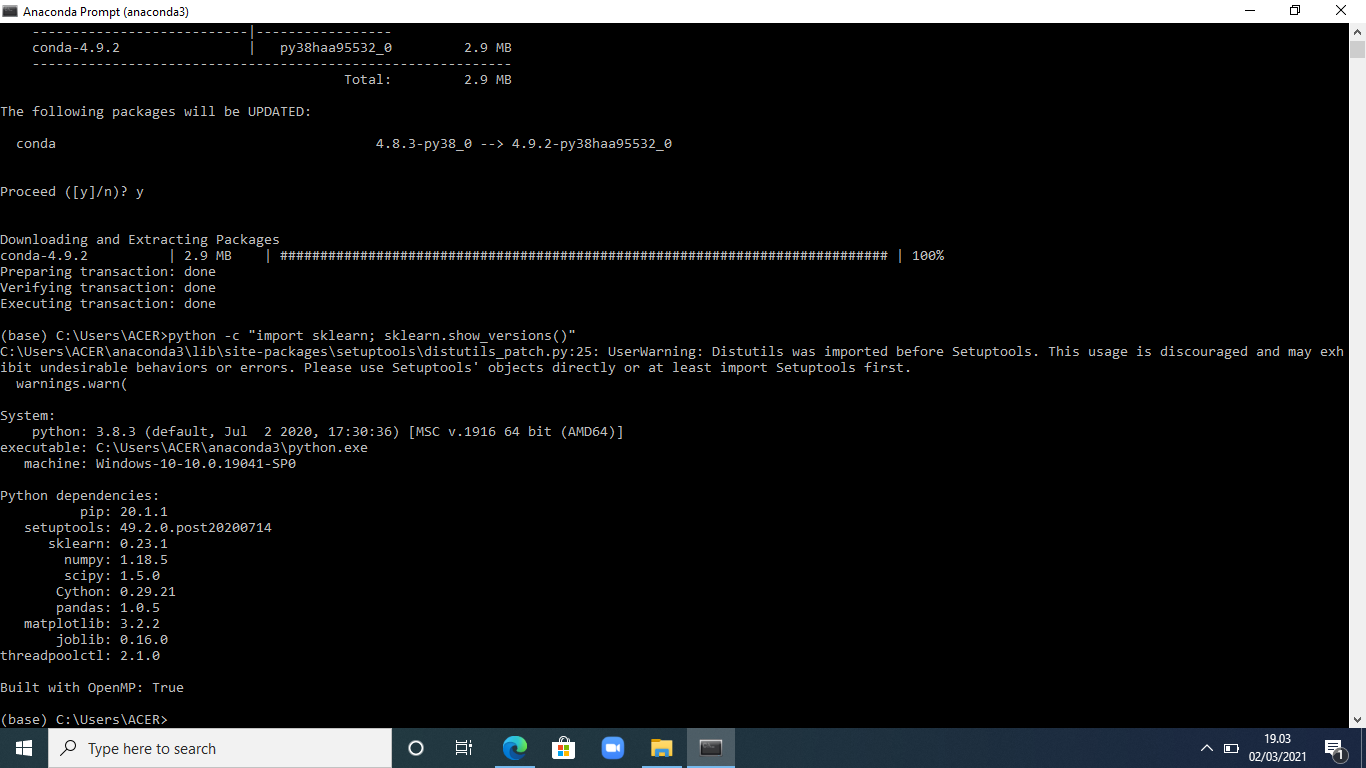
\includegraphics[width=10cm]{figures/1184003/chapter1/1.png}
		\centering
		\caption{Instalasi Library Scikit Learn}
	\end{figure}
	\begin{figure}[h]
		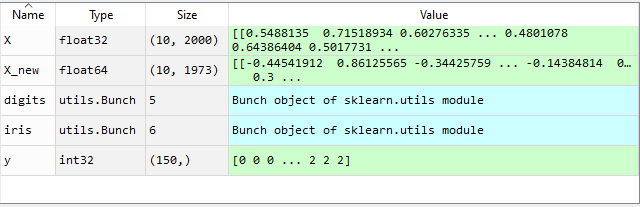
\includegraphics[width=10cm]{figures/1184003/chapter1/2.PNG}
		\centering
		\caption{Isi Variabel Explorer}
	\end{figure}
	\newpage\item Uji coba loading an example dataset
	\hfill\break
\lstinputlisting[firstline=7, lastline=16]{src/tugas1.py}
\item Uji coba Learning dan predicting
	\hfill\break
	\lstinputlisting[firstline=17, lastline=32]{src/tugas1.py}
\item Uji coba Model Persistence
	\hfill\break
	\lstinputlisting[firstline=35, lastline=63]{src/tugas1.py}	
	\item Uji coba Conventions
	\hfill\break
	\lstinputlisting[firstline=64, lastline=82]{src/tugas1.py}
	\end{enumerate}
	\subsection{Penanganan Error}
\begin{enumerate}
	\item ScreenShoot Error
	\begin{figure}[h]
		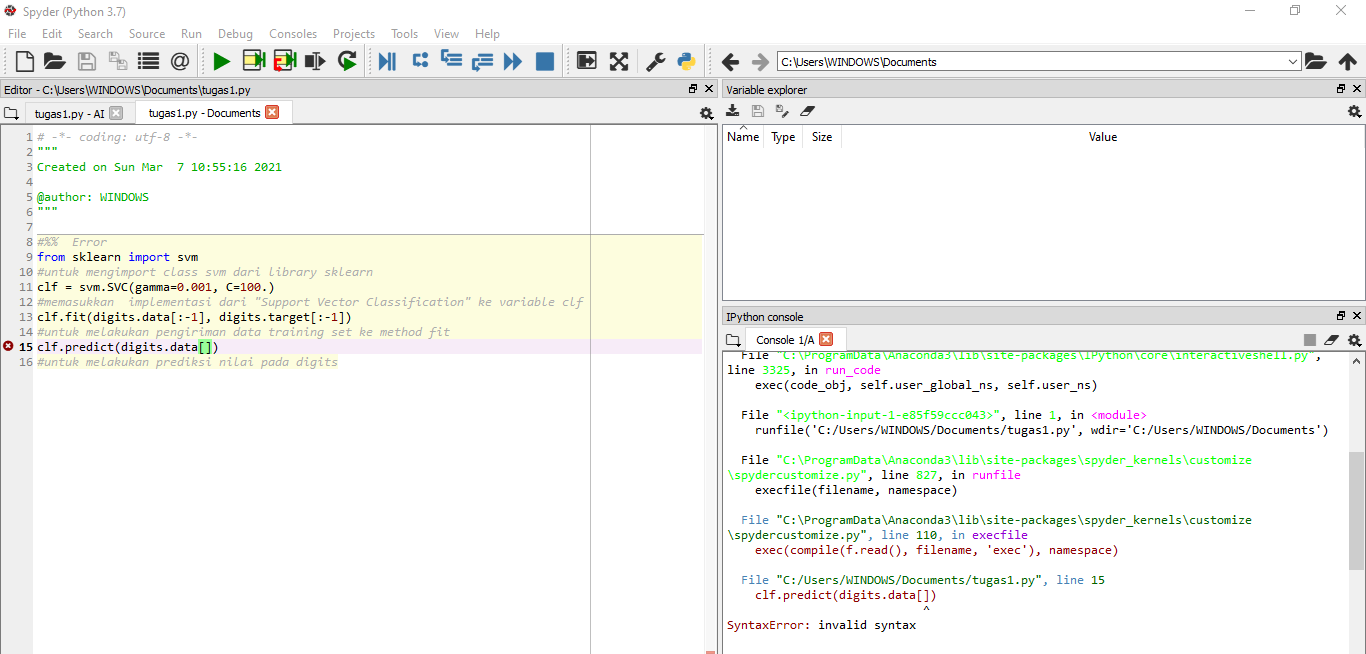
\includegraphics[width=10cm]{figures/1184003/chapter1/3.PNG}
		\centering
		\caption{Name Error}
	\end{figure}
	\newpage\item Tuliskan Kode Error dan Jenis Error
	\hfill\break
	\lstinputlisting[firstline=83, lastline=91]{src/tugas1.py}
\hfill\break
	\item Cara Penangan Error
\hfill\break Tambahkan prediksi nilainya agar kode program dapat terbaca
	\end{enumerate}
	\subsection{Bukti Tidak Plagiat}
\begin{figure}[h]
	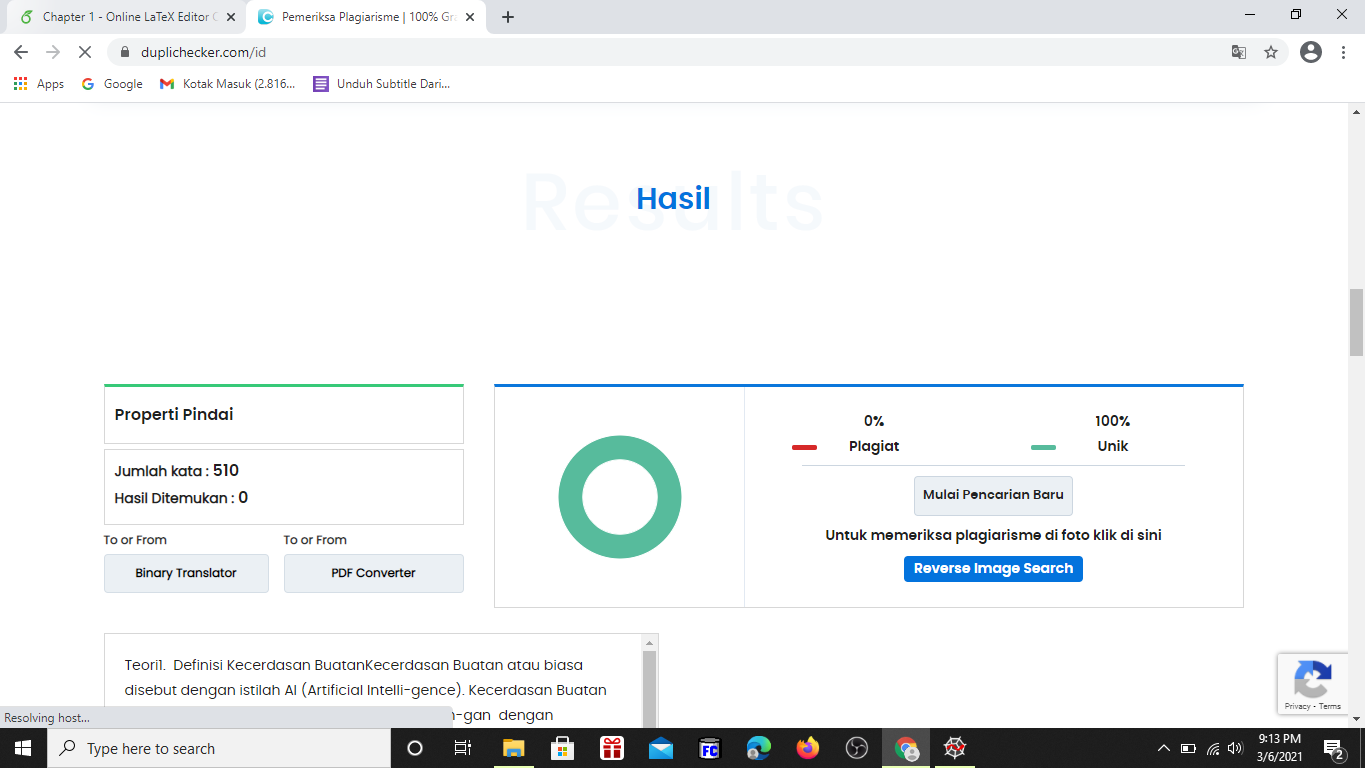
\includegraphics[width=10cm]{figures/1184003/chapter1/4.png}
	\centering
	\caption{Bukti Tidak Melakukan Plagiat Chapter 1}
\end{figure}